\documentclass[../main.tex]{subfiles}
\begin{document}

\section{模型建立和求解}

\subsection{问题1}
\subsubsection{模型准备}
\paragraph{三维热传导方程的推导}
热传导源自温度的不均匀分布,热传导的强弱程度可以用热流强度 \(\vec{q}\),也就是单位时间内通过单位横截面积的热量来进行刻画,温度的不均匀程度可以用温度梯度 \(\nabla u\) 来进行刻画,其中 \(u\) 指的是温度。

傅里叶定律指出,热流强度和温度梯度 \(\nabla u\) 成正比,也就是
\begin{equation}\label{equ:fou}
\vec q = - k \nabla u
\end{equation}
考虑三维空间之中的热量传导,设热源强度,也就是单位时间内在单位体积内部产生的热量为 \(F (x,  y , z, t)\),任取一体积微元 \(\Omega\),应用能量守恒定律有:
\begin{equation}
\oiint _{\, \Omega} \vec q \cdot \mathrm{d} S = \oiiint _{\, \Omega} ( F (x , y , z,t) - u _{t} c \rho ) \, \mathrm{d} V
\end{equation}
其中 \(c\) 是体积微元的比热容,\(\rho\) 为体积微元的密度。

根据散度定理
\begin{equation}
\oiint _{\,\Omega} \vec A  \cdot \mathrm{d} S = \oiiint _{\,\Omega} ( \nabla\kern -1.8pt\vec A) \, \mathrm{d}V
\end{equation}
将其和Equ~(\ref{equ:fou}) 联立可得
\begin{equation}
\nabla \vec q = F (x , y , z ,t) - u_{t} c \rho
\end{equation}
再代入 Equ~(\ref{equ:fou}) 即可得到三维热传导方程:
\begin{equation}\label{equ:cond}
u_{t} c \rho - k\kern 1pt \nabla^{2} u = F (x , y , z, t)
\end{equation}
% TODO 其中 \(k\) 是什么?

\paragraph{牛顿冷却定律}
牛顿冷却定律指出,两个不同温度的介质之间发生热对流的时候,热流强度和两个介质之间的温度差成正比,也即
\begin{equation}
\vec q = h (u_1 - u_2)
\end{equation}
其中 \(u_1\) 所在的介质指向 \(u_2\) 所在介质的方向向量在 \(\vec q\) 所规定的正方向上具有正分量,将其代入Equ~(\ref{equ:fou}),即得:
\begin{equation}\label{equ:len}
{-k} \nabla u = h ( u_1 - u_2)
\end{equation}
% subsubsection:模型准备

\subsubsection{模型建立}
% para one
\paragraph{复原间隙温度} 先是复原间隙以及炉前后区域之中的温度,用 \(u\) 表示。

对于两个温区之间的间隙,其只受到两边温区的加热,并且间隙之中并没有热源,三维热传导方程Equ~(\ref{equ:cond})中 \(F ( x , y , z ,t) = 0\),且退化为一维热传导方程:
\begin{equation}
\frac{\partial u}{\partial t} = a^{2} \frac{\partial ^{2} u}{ \partial x ^{2}}
\end{equation}
% TODO 在这里 \(a\) 是什么?
考虑到温度已经稳定,也就是温度不再变化,也就是 \(\frac{\partial u}{ \partial t} = 0\), 于是有 \(\frac{\partial ^{2} u}{\partial x ^{2}} = 0 \),
也即,间隙中的温度关于 \(x\) 是线性变化的。于是说给定了两边温区的温度之后,假设是 \((x_1, T_1), (x_2, T_2)\), 就能够得出间隙中的温度关于距离 \(x\) 的表达式:
\[
u(x)  = T_{1} + \frac{T_2 - T_1}{x_2 - x_1} \cdot x
\]
能够根据温区的温度给出炉内上下表面的温度曲线。对于附件所描述的某次实验,\(T _{1 \sim 5} = 17 5 ^{\circ}\mathrm{C}\), \(T _{6} = 195 ^{\circ}\mathrm{C}\), \(T _{7} = 235 ^{\circ}\mathrm{C}\), \(T _{8 \sim 9} = 255 ^{\circ}\mathrm{C}\),以炉前区域最左端为\(x\)起点,能够得到温度 \(u\) 关于距离 \(x\) 的函数图像,见图~\ref{fig:1},温度 \(u\) 关于距离 \(x\) 的函数记为 \(u ^{\dagger}\)。
\input pic.tex

% para
\paragraph{温度分布方程的导出}
不妨设炉内的温度分布为 \(u ( x,  y  ,z ,t)\),由于炉内的温度沿着 \(z\) 轴对称分布,因此为 \(\frac{\partial u}{ \partial z} = 0\)。由题意,回焊炉启动之后,颅内空气温度会在短时间内达到稳定,因此 \( \frac{\partial u}{ \partial t} = 0\)。代入三维热传导方程Equ~(\ref{equ:cond})得:
\begin{equation}
0 - k \bigg( \frac{\partial ^{2} u }{\partial x ^{2}} + \frac{\partial ^{2} u}{\partial x ^{2}} + 0\bigg) = F (x , y, z , t)
\end{equation}
又由于考察的区域为不包含温区的传动带区域,因此 \(F (x, y , z , t) = 0\),故上式转化为:
\begin{equation}
\frac{\partial ^{2} u}{\partial x ^{2}} + \frac{\partial ^{2} u}{\partial y ^{2}} = 0
\end{equation}
能够知道 \(u\) 只是 \(x , y\) 两个维度的函数,且满足拉普拉斯方程。

由于 \(u\) 不是关于 \(t\) 的函数,故不必考虑方程的初始条件
考察温区间隙的温度分布 \(u (x,  y , z ,t)\)。根据模型假设,温区间隙的热流仅沿 \(x\) 轴方向传播,则对于间隙有,\(\frac{\partial u}{\partial y} = 0\)。与炉内同理,\(\frac{\partial u}{ \partial z} = 0\),\(\frac{\partial u}{\partial t} = 0\),\(F(x, y , z,t) = 0\)。可知\(u\)仅为 \(x\) 的函数。代入三维热传导方程 Equ~(\ref{equ:cond}),有:
\begin{equation}
0 - k \bigg( \frac{\partial ^{2} u}{ \partial x ^{2}} + 0 + 0\bigg) = 0
\end{equation}
也就是
\begin{equation}
\frac{\partial ^{2} u}{\partial x ^{2}} = 0
\end{equation}
由于 \(u\) 是关于 \(x\) 的函数,可知 \(u = kx + b\),即温度为 \(u_{1} , u_2\) 的两个温区的间隙的温度分布为 \(u = \displaystyle \frac{u_2 - u_1}{\varDelta d} ( x - x_1) + u_1\),其中 \(\varDelta d\) 是间隙的长度。

于是,视炉前区域、炉后区域为第\(0\), 12 个小温区,假设第\(i\)个小温区的温度为 \(u_{i}\),左右两侧作坐标为 \(x_{il}\), \(x_{ir}\),并且假设上下两个温区之间间距为 \(l\),炉前区域、炉后区域之间间距为 \(l_{0}\),则炉内温度分布的边界条件为
\begin{equation}
\begin{cases}
u|_{y = \pm l/2} =
\begin{cases}
\frac{u_{i+1} - u_{i}}{\varDelta d} (x - x_{ir}) + u_{i} , & \quad x _{ir} < x < x_{i+1 l} \\
u_{i} = 25 ^{\circ}\mathrm{C}, & \quad  x_{il} \le x \le x_{ir}
\end{cases} \\
u|_{x = 0} = 25 ^{\circ}\mathrm{C}\\
u|_{x = l_{0}} =  25 ^{\circ}\mathrm{C}
\end{cases}
\end{equation}
综上,回焊炉内部的温度分布方程为
\begin{equation}
\begin{cases}
\displaystyle\frac{\partial ^{2} u}{\partial x ^2} + \frac{\partial ^{2} u}{\partial y ^{2}} = 0\\
u|_{y = \pm l/2} =
\begin{cases}
\displaystyle\frac{u_{i+1} - u_{i}}{\varDelta d} (x - x_{ir}) + u_{i} , & \quad x _{ir} < x < x_{i+1 l} \\
\displaystyle u_{i} = 25 ^{\circ}\mathrm{C}, & \quad  x_{il} \le x \le x_{ir}
\end{cases} \\
u|_{x = 0} = 25 ^{\circ}\mathrm{C}\\
u|_{x = l_{0}} =  25 ^{\circ}\mathrm{C}
\end{cases}
\end{equation}
% TODO

%% para
\paragraph{拉普拉斯方程的数值求解} 根据逐次超松弛迭代法,使用网格化分割方法,可以列出如下迭代方程
\begin{equation}
u_{k,j} ^{(i)} = \frac{\beta}{4} \bigg( u_{k-1, j} ^{(i)} + u_{k,j-1} ^{(i)} + u_{k+1,j} ^{(i-1)}+ u _{k, j+ 1} ^{(i-1)} \bigg) + (1- \beta) u_{k,j} ^{i-1} ,\quad \beta \in (1, 2]
\end{equation}
其中 \(i\) 为迭代次数,可以绘制出下面 \(u ( x , y)\) 图像

\begin{figure}[H]
\centering
\includegraphics[scale = 0.5]{fig1.pdf}\caption{什么图像}
\end{figure}
% TODO

%% para
\paragraph{确定热传导方程} 对于中间部分的焊接材料,设其在受到加热的时候温度为 \(v\),热传导率为 \(k\),密度为 \(\rho\),比热容为 \(c\),此时空气和焊锡之间的热对流系数为 \(h\),于是三维热传导方程Equ~(\ref{equ:cond})之中的 \(F (x, y , z, t)\) 满足 \(F ( x , y , z ,t ) = 0\),由于焊接材料只在厚度这一个方向上传热,于是三维热传导方程退化为在 \(y\) 轴方向上传热的热传导方程,也即
\begin{equation}\label{equ:one-dim}
\frac{\partial v}{\partial t} - a ^{2} \frac{\partial^{2} v }{\partial y ^{2}} = 0
\end{equation}
% TODO 其中 \(a\) 是?

初始时,其温度为车间温度,也即,当时刻为零的时候,\(v\) 的值为 \(25 ^{\circ}\mathrm{C}\)。
\begin{equation}
v (y, 0) = 25 ^{\circ}\mathrm{C}, \quad y \in [0, {\it height}\kern 1pt]
\end{equation}
在这里将 \(v\) 视为两个参数的函数,接收 \(y\) 轴方向上的坐标\(y\)以及时间 \(t\)。

由于焊接材料仅在 \(y\) 轴一个方向上传热,傅里叶热传导方程 Equ~\ref{equ:fou} 可以退化为
\begin{equation}
\vec q = {-} k \frac{\partial v}{ \partial y}
\end{equation}
将 \(\vec q\) 代入牛顿冷却定律Equ~\ref{equ:len},并对焊接材料两端和空气之间的热对流过程进行分析,可得边界条件:
\begin{equation}\label{equ:bian}
\begin{cases}
\displaystyle- k \left.\frac{\partial v}{\partial y}\right|_{y = 0} =  h \Big[ u(t) - v(0, t)\Big] \\
\displaystyle- k \left.\frac{\partial v}{\partial y}\right|_{y = {\it height}} = h \Big[v({\it height}, t) - u(t)\Big]
\end{cases}
\end{equation}
其中\(u(t)\) 是对应时刻,焊接材料表面的空气温度。\(u ^{\dagger}\) 为温度关于距离 \(x\) 的函数,在上文之中已经求出,则 \(u (t) = u^{\dagger} ( Vt)\),其中 \(V\) 是过炉速度。
综上,可对热传导模型建立如下方程:
\begin{equation}
\begin{cases}
\displaystyle \frac{\partial v}{\partial t} - a ^{2}  \frac{\partial ^{2} v}{\partial y^{2}} = 0 \\
\displaystyle v (y , 0) = 25 ^{\circ}\mathrm{C}, \quad y \in [0, {\it height\kern 1pt}] \\
\displaystyle- k \left.\frac{\partial v}{\partial y}\right|_{y = 0} =  h \big[u(t) - v(0, t)\big] \\
\displaystyle- k \left.\frac{\partial v}{\partial y}\right|_{y = {\it height}} = h \big[v({\it height}, t) - u(t)\big]
\end{cases}
\end{equation}

%%
\paragraph{差分形式}
将边界条件差分化,对于任意时刻,有
\begin{equation}
\begin{cases}
\displaystyle - H \cdot \frac{v _{1, t}  - v _{0, t}}{\mathrm{dy}} + v_{0 ,t} = u_{t} \\
\\
\displaystyle H \cdot\frac{v_{M , t} - v _{M-1, t}}{\mathrm{dy}} + v_{M,t} = u_{t}
\end{cases}
\end{equation}
其中 \(H = \dfrac{k}{h}\),\(\mathrm{dy}\) 是距离步长,\(v_{i,j}\) 是焊接材料温度 \(v\) 离散化后的结果,\(i\) 为距离指标 \(i = 0,  1,  2 , \dots , M\), \(j\) 是时间指标 \(j = 0 , 1 , 2 , \dots, N\)。对上式子进行化简能够得到:
\begin{equation}
\begin{cases}
\displaystyle v_{0,t} = \frac{H}{H + \mathrm{dy}} v_{1 ,t} + \frac{\mathrm{dy}}{H + \mathrm{dy}} \cdot u_{t}\\
\\
\displaystyle v_{M,t} = \frac{H}{H + \mathrm{dy}} v _{M-1, t} + \frac{\mathrm{dy}}{H + \mathrm{dy}} \cdot u_{t}
\end{cases}
\end{equation}
而对于焊接材料的一维热传导方程 Equ~(\ref{equ:one-dim})进行差分化,能够得到一个半差分形式:
\begin{equation}
\frac{\partial v _{i}}{\partial t} = a \cdot \frac{u_{i+1, t} - 2 u_{i, t} + u_{i- 1 , t}}{\mathrm{dy} ^{2}}
\end{equation}
在这里时间差分采用向后欧拉法,得到全差分格式如下:
\begin{equation}\label{equ:all}
\frac{\mathbf{v}_{t+1}  - \mathbf{v}_{t}}{\tau}= \frac{a}{\mathrm{dy}^{2}} (\mathbf{A}\mathbf{v} _{t+1} + \mathbf{b})
\end{equation}
其中 \(\tau\) 是时间步长,\(\mathbf{v}_{t}\) 是一个向量,其值为 \([v _{1, t}, v_{2, t}, \dots, v_{M, t}]^{\mathrm{T}}\),也即,时间指标为 \(t\) 的时候焊接材料上面各个点温度所组成的向量,其中矩阵\(\mathbf A\) 满足
\begin{equation}
\mathbf{A} =
\begin{bmatrix}
\frac{H}{H + \mathrm{dy}} - 2 & 1 &&\\
\\[-10pt]
1 & -2 & 1 &\\
& & 1 & -2 & 1 \\
\hdotsfor{6}\\
\\[-10pt]
&& & 1 & -2 & 1 \\
\\[-10pt]
&& &  & 1 &\frac{H}{H + \mathrm{dy}} -2
\end{bmatrix}
\end{equation}
并且 \(\mathbf{b} = \displaystyle \bigg[ \frac{\mathrm{dy}}{H + \mathrm{dy}} \cdot u_{t} , 0 ,\dots, 0 , \frac{\mathrm{dy}}{H + \mathrm{dy}} \cdot u_{t} \bigg] ^{\mathrm{T}}\)。
令 \(r = \displaystyle \frac{a \tau}{h ^{2}}\),随后根据全差分形式~\ref{equ:all},化简得到
\begin{equation}\label{equ:iter}
(\mathbf{I} - r\mathbf{A} ) \mathbf{v} _{t+1} = \mathbf{v}_{t} + r \mathbf{b}
\end{equation}
本文使用迭代形式 Equ~(\ref{equ:iter}) 进行 \(\mathbf{v}_{t}\) 的迭代。

对于 \(\mathbf{I} - r \mathbf{A}\),其值为
\begin{equation}
\mathbf{I} - r \mathbf{A} =
\begin{bmatrix}
1 - \big(\frac{H}{H + \mathrm{dy}}\big) r & -r \\
-r & 1 + 2r & -r \\
\hdotsfor{5}\\
&&-r & 1 + 2r & -r \\
&&& -r & 1 - \big(\frac{H}{H + \mathrm{dy}}- 2\big)r
\end{bmatrix}
\end{equation}

%% par
\paragraph{分段拟合} 考虑到焊接材料的性质会根据材料本身的温度发生改变,在不同区域内部焊接材料的热扩散系数\(A\)和焊接材料和空气之间的热对流交换系数\(h\)也不同,本文将整个加热过程分为三段,假设每一段之中热扩散系数和热对流交换系数不发生改变,这三段的系数表示为 \(A_{i}, h_{i}\), \(i = 1 , 2 ,3 \),并进行分段拟合求出 \(A_{i} ,h_{i}\)。

本文将加热过程按照炉温的高低分为三段:低温区、高温区和冷却区:
\begin{table}[H]
\centering
\begin{tabular}{ccc}
编号&区域 & 范围 / cm \\ \hline \hline
\\ [-1em]
I&低温区& \([0 , 200]\) \\
II&高温区& \([200, 342]\) \\
III&冷却区& \([342, 435.5]\)
\\ [-1em]
\\ \hline
\end{tabular}\caption{根据炉温划分的区域}
\end{table}
低温区是炉前区域的最左端到第五个小温区和第六个小温区之间的间隙的中点,高温区是低温区末端到第九个小温区和第十个小温区之间的间隙的中点,剩余部分便是冷却区。

本文先是对低温区域进行拟合,得出低温区的焊接材料的参数,也就是 \(A_{1}, h_{1}\)。得到的低温区域末端的温度作为高温区的初始条件,同样进行拟合,得到高温区的焊接材料的参数 \(A_{2}, h_{2}\)。同理得到 \(A_{3}, h_{3}\)。拟合得到的结果如下表
\begin{table}[H]
\centering
\begin{tabular}{ccc}
& \(A_{i}\) \(\mathrm{W}/ (\mathrm{m}\cdot \mathrm{K})\) & \(h_{i}\) \(\mathrm{W} / (\mathrm{m}^{2} \cdot \mathrm{K})\) \\ \hline \hline
\\[-1em]
I & \(5 \times 10 ^{-11}\) & \(5 \times 10 ^{-6}\) \\
II & \(6 \times 10 ^{-11}\) & \(4 \times 10 ^{-7}\) \\
III & \(3 \times 10 ^{-11}\) & \(1 \times 10 ^{-5}\)
\\[-1em]
\\ \hline
\end{tabular}\caption{焊接材料在不同区域内拟合出的参数}
\end{table}

% subsubsection:模型建立
\subsection{问题2}
根据题意,找到的最大的过炉速度 \(V\) 需要满足下面条件,焊接材料的中心位置的温度 \(v\)是关于时间\(t\)的函数,有:

\begin{table}[H]
\centering
\begin{tabular}{ccccc}
编号&限制 & min & max 	& 单位
\\ [-1em]
\\ \hline \hline
\\ [-1em]
1&\(\vert v '\vert\) & 0 & 3 & \(^{\circ}\mathrm{C} / \mathrm{s}\)\\
2&处于 \(150 ^{\circ}\mathrm{C}\sim 190 ^{\circ}\mathrm{C}\) 的时间 & 60 & 120 & \(\mathrm{s}\)\\
3&大于 \(217 ^{\circ}\mathrm{C}\) 的时间 & 40 & 90 & \(\mathrm{s}\)\\
4&\(\max {v}\) & 240 & 250 & \(^{\circ}\mathrm{C}\)
\\ [-1em]
\\ \hline
\end{tabular}
\end{table}

以下本文分析四个限制指标与过炉速度之间的关系,得到四张函数图像,见图~\ref{fig:four}。
\begin{figure}[H]
\centering
	\begin{subfigure}[b]{0.4\textwidth}
		\centering
		\includegraphics[width=\textwidth]{k.pdf}
		\caption{\(\vert v' \vert\) 的最值}
	\end{subfigure}
	%
	\begin{subfigure}[b]{0.4\textwidth}
		\centering
		\includegraphics[width=\textwidth]{190170.pdf}
		\caption{处于\(150 ^{\circ}\mathrm{C}\)\(\sim\)\(190 ^{\circ}\mathrm{C}\)的时间}
	\end{subfigure}
	%
	\begin{subfigure}[b]{0.4\textwidth}
		\centering
		\includegraphics[width=\textwidth]{217.pdf}
		\caption{大于 \(217 ^{\circ}\mathrm{C}\)的时间}
	\end{subfigure}
	%
	\begin{subfigure}[b]{0.4\textwidth}
		\centering
		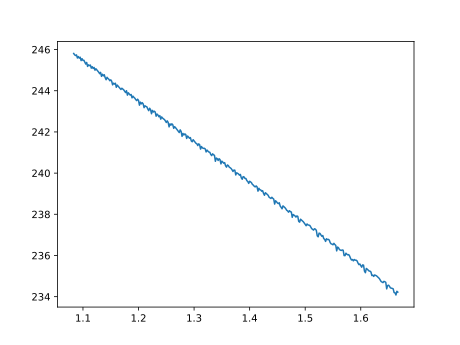
\includegraphics[width=\textwidth]{max.pdf}
		\caption{\(v\) 的峰值}
	\end{subfigure}
	\caption{四个限制指标和过炉速度之间的关系}\label{fig:four}
\end{figure}
由图可知,这四个指标与过炉速度满足单调函数关系,因此本文拟通过二分法求解最大过炉速度,二分法的递归伪代码如下给出:
\begin{minted}[linenos, fontsize = \footnotesize]{python}
def  BinarySerach(Tlist, Vlist, low, high):
  if  high > low:
    mid = (low + high) // 2

    # 当最大斜率过大时,向慢速搜索
    maxK = searchMaxK(Tlist, Vlist[mid])
    if maxK > 3:
       return BinarySerach(Tlist, Vlist, low, mid-1)

    # 当峰值温度过小时,向慢速搜索
    maxTemp = searchMaxTemp(Tlist, Vlist[mid])
    if maxTemp < 240:
      return BinarySerach(Tlist, Vlist, low, mid-1)
    if maxTemp > 250:
      return BinarySerach(Tlist, Vlist, mid+1, high)

    # 当超过217摄氏度的时间越短时,向慢速搜索
    Lt217times = searchLt217times(Tlist, Vlist[mid])
    if  Lt217times < 40:
      return BinarySerach(Tlist, Vlist, low, mid-1)
    if  Lt217times > 90:
      return BinarySerach(Tlist, Vlist, mid+1, high)

    # 当从150度上升至190度的时间越短时,向慢速搜索
    Uptimes = searchUptimes(Tlist, Vlist[mid])
    if  Uptimes < 60:
      return BinarySerach(Tlist, Vlist, low, mid-1)
    if  Uptimes > 120:
      return BinarySerach(Tlist, Vlist, mid+1, high)

    # 满足问题需要,当满足所有条件时,向快速搜索
    # 便于获得最大过炉速度
    return BinarySerach(Tlist, Vlist, mid, high)
  else:
    return Vlist[low]
\end{minted}
通过二分搜索模型,本文最终确定的最大过炉速度为\(82.47 \mathrm{cm}/\mathrm{min}\)。

\subsection{问题 3}
\subsubsection{模型准备}
% para
\paragraph{十进制蚁群算法的原理}
针对问题3中最优炉温曲线的求解,易知是一个多元连续函数优化问题。以理想的炉温曲线应使超过\(217 ^{\circ}\mathrm{C}\)到峰值温度所覆盖的面积最小的目标函数如下:
\begin{equation}
\min S = \mathrm{getSquare} (T _{1 {\sim} 5},T _{6} , T _{7} , T _{8 {\sim} 9}, V) \\
\end{equation}
约束条件为
\begin{equation}{\it s.t.}
\begin{cases}
V = \mathrm{binarySearchMaxV} (T _{1{\sim} 5}, T_{6} , T _{7},T_{8{\sim} 9})\\
165 \le T_{1 {\sim} 5} \le 185\\
185 \le T _{6} \le 205 \\
225 \le T _{7} \le 245 \\
245 \le T _{8 {\sim} 9} \le 265
\end{cases}
\end{equation}
本文拟采取十进制蚁群算法,对各温区温度进行搜索。

以下本文将以一元连续函数为例,说明十进制蚁群算法的原理。设一元连续函数优化的数学模型如下:
\begin{equation}
\min f(x), \quad x \in [x_1 , x_2]
\end{equation}
%
\begin{enumerate}
	% one item
	\item 转换决策变量区间\\
	通过一个映射函数将\(x\)的变化区间从\([x_1,x_2]\)变换到\([0,1]\)区间上,设决策变量的精度是\(d\),即变换后的\(x\)具有\(d\)位十进制小数。
	\smallskip
	% one item
	\item 构建城市群\\
	对于变换后的决策变量\(x\),构建规格为 \(1+10\times d\) 的城市群。其中``1''代表个位数``0'',第``d''列代表小数点后第\(d\)位有效数字,``10''行表示每位小数有\(0 {\sim} 9\)这十个十进制数的取值。城市群示意图如下:
	\smallskip
	%
	\begin{figure}[H]
	\centering
	\includegraphics[scale = 0.5]{cities.png}
	\caption{十进制蚁群算法城市群示意图}\label{fig:cities}
	\end{figure}
	% one item
	\item 蚂蚁移动路径通过解码获得可行解\\
	规定每一只蚂蚁的移动路径遵循以下原则:
	\begin{itemize}
		\item 蚂蚁只能从最左端的起点出发;
		\item 蚂蚁必须从左向右移动,每一次路径选择,也就是在选择下一列城市时只允许在一个城市上落脚;
		\item 当蚂蚁移动到最后一列的时候,其从第0列移动到第\(d\)列一共移动了 \(1 + d\) 个城市,通过这些城市各自所在的列 \((0 {\sim} 9)\) 和编号 \(( 0 {\sim} 9)\)获得 \([0,1]\)上的十进制可行解。
	\end{itemize}
	\smallskip
	% one item
	\item 路径转移以及信息素更新
	\begin{enumerate}
		% two item
		\item 路径转移\\
		记第 \(r\) 列第 \(i\) 城市到第 \(r+ 1\) 列第 \(j\) 城市之间的路径为 \(\mathrm{Path} _{ij} ^{r}\),第 \(r\) 列第 \(i\) 城市到第 \(r+ 1\) 列第 \(j\) 城市之间的信息素浓度 \(\tau ^{r} _{ij}\),其中 \(r = 1, 2, \dots , d\); \(i = 0, 1 , \dots , 9\); \(j = 0 , 1 , \dots , 9\)。通过生物学中对于蚂蚁习性的研究,十进制蚁群算法中将蚂蚁从第 \(r\) 列第 \(i\) 城市转移到第 \(r+1\) 列第 \(j\) 城市的概率简化为以下形式:
		\begin{equation}\label{equ:pass1}
		\rho _{ij} ^{r} = \frac{\tau ^{r} _{ij}}{\sum\limits_{s\in \{0 , \dots , 9\}} \kern -2pt\tau ^{r} _{is}}
		\end{equation}
		城市转移到第r+1列中的10个城市中,路径 \(\mathrm{Path}_{ij} ^{r}\)的信息素浓度越高,转移到城市 \(j\) 的概率就越大。在没有完全排除其余路径的基础上,这样的转移方式不仅保证了更多的蚂蚁样本将被聚集到当前的最优路径,符合最优搜索策略的原则,还有利于帮助小部分蚂蚁寻找其他更优路径,在有其他更好的选择的情况之下跳出局部最优的限制。
		\smallskip
		% two item
		\item 信息素更新\\
		当第 \(N\) 轮次的循环结束时,所有蚂蚁将在自身移动过的路径上留下信息素增量,与前一轮次挥发后剩余的信息素叠加获得该轮次的信息素矩阵:
		\begin{equation}\label{equ:shit}
		T_{N} = (1 - \rho) T _{(N- 1)} + \Delta T
		\end{equation}
		\(T_{N}\) 是一个三维信息素矩阵,存放着\(d\) 个从第 \(0\sim d -1\) 列的第 \(i\) 城市转移到下一列第\(j\)城市的二维信息矩阵 \(S_{ij}\);\(N\) 代表当前循环轮次;\(\rho\) 表示挥发系数,其取值越大,挥发强度就越高,前一轮次留下的信息素残余量对当前轮次蚂蚁的路径转移影响就越小,项最优解收敛的速度就越快。
		\(\Delta T\) 代表当前轮次的信息素增量,本文采用精英策略对每一只蚂蚁留下的信息素进行取值:

		\begin{itemize}
			% third item
			\item[\rom{1}] 在一轮次循环结束之后,通过排序取得前 \(\alpha \%\)的精英蚂蚁,这些精英蚂蚁各自路径上的信息素增量为
			\begin{equation}\label{equ:pass2}
				\Delta \tau _{ij} = K Q ^{J [f (x_{k}) - f (x _{\mathrm{best}})]} , \quad (k \le \alpha \% \cdot \mathrm{num}_{\mathrm{ant}} , k \in \mathbf{Z})
			\end{equation}
			其中\(\mathrm{num}_{\mathrm{ant}}\)为蚂蚁总数量,\(K\)为信息素权值系数,同时也是最优解路径对应的增量值;\(J\)为放缩系数,可以把函数值差值进行无量纲化到一个合理的区间内;\(x_{\mathrm{best}}\)是这些精英解中的最优解,\(Q\)系数的取值为\((0,1)\),这个幂项将根据每个可行解与最优解的目标函数值距离,降低其信息素增量值。函数值越接近最优解值,降低的幅度就越小,对应的信息素增量就越大。
			\smallskip
			% third item
			\item[\rom{2}] \(\alpha \%\)后的蚂蚁,其信息素增量置为0。
			\smallskip
			% third item
			\item[\rom{3}] 同时,为了增强该模型的局部搜索能力(local search ability),提高搜索效率和精度,当在最优路径上的信息素增量为\(\Delta \tau\)时,其相邻的路径上也对应着增加\(\Delta \tau / 4\)的信息素增量。\\
			例如当最优解是 0.40 时,即\(\Delta \tau _{0 4} ^{0} = \Delta \tau ^{1} _{4 0} = \Delta \tau\)时,局部搜索模型将对0.3,0.5,0.39,0.41处的信息素增量\(\Delta \tau ^{0} _{03}, \Delta \tau_{05} ^{0} , \Delta \tau _{39} ^{1} , \Delta\tau _{41}^{01}\)加上\(\Delta \tau / 4\)。
			通过这样的方法,当前最优路径附近上的更优路径将有更大的概率被搜索到。
			\end{itemize}
		\end{enumerate}
	% one item
	\item 从一元连续函数推广到多元连续函数优化的十进制蚁群算法\\
	对于含有\(k\)个决策变量的多元连续函数,构建含有
	\(\sum_{i = 1} ^{k} (1+ 10 d_{i})\)个城市的城市群,每个决策变量对应一个子城市群,每个子城市群的最后一列城市上的蚂蚁将转移到下一子城市群的第0列的城市上。其余路径转移与信息素更新规则都与一元连续函数保持一致。
\end{enumerate}
% subsubsection:模型准备

\subsubsection{模型建立}
以下给出蚁群算法的具体实现步骤:
\begin{enumerate}
	\item 设置初始参数:
	蚂蚁数量 \(\mathrm{num}_{\mathrm{ant}}\); 循环次数\(\mathrm{loop}_{\mathrm{times}}\); 各个参数的精度\(d_i\); 挥发系数\(\rho\); 调节系数\(J\)、\(Q\)、\(K\); 精英占比\(\alpha  \%\); 所有路径信息素初值\(τ_0\)。
	\item 对于每一只蚂蚁,根据路径转移公式Equ~(\ref{equ:pass1})计算每只蚂蚁的转移概率,根据转轮盘法确定蚂蚁所选择的下一路径城市。重复该操作直到所有蚂蚁完成一次循环。
	\item 对于蚂蚁路径进行解码获得可行解,通过计算目标函数值,确定精英策略下的精英蚂蚁较优解,根据公式Equ~(\ref{equ:pass2})和局部搜索增强策略获得对应的信息素增量矩阵,再由Equ~(\ref{equ:shit})更新获得新一轮的信息素矩阵。
	\item 当循环结束时,返回每一个决策变量所对应的子城市群中信息素浓度最高的路径即获得十进制蚁群算法的最优解。
\end{enumerate}
\begin{table}[H]
	\centering
	\begin{tabular}{cccccccc}
	\hline 	\hline
	\\[-1em]
	\(\mathrm{num}_{\mathrm{ant}}\) & \(\mathrm{loop}_{\mathrm{times}}\) & \(K\) & \(Q\) & \(J\) & \(\rho\) & \(\alpha\%\) & \(d_{i}\) \\
	\\[-1em]
	\hline
	\\[-1em]
	\(100\)  & \(10\)  & 5  & 0.8  & 100  & 0.4  & 10\%  & 1
	\\[-1em]
	\\ \hline
	\end{tabular}
	\caption{十进制蚁群算法参数设置}
\end{table}
最终确定的最佳温度控制为 \(T _{1 \sim 5}= 183 ^{\circ}\mathrm{C}\),\(T6 = 187^{\circ}\mathrm{C}\),
\(T_{7} = 235^{\circ}\mathrm{C}\),\(T_8 = 255^{\circ}\mathrm{C}\),最佳过炉速度为 \(90\,\mathrm{cm}/\mathrm{min}\),炉温曲线超过\(217 ^{\circ}\mathrm{C}\)到峰值温度所覆盖的面积为\(435\,^{\circ}\mathrm{C} \cdot \mathrm{min}\)。
% subsubsection:模型建立
\end{document}
